\documentclass{article}
\usepackage[bottom]{footmisc}
\usepackage{graphicx}
\usepackage{float}
\usepackage{titlesec}
\usepackage{amsmath}
\usepackage{hyperref}
\usepackage{makeidx}

\setcounter{secnumdepth}{4}

%\usepackage{adjustbox}  
\newcommand{\V}{\verb}
\newcommand{\x}{$\textbf{X}$}
\newcommand{\y}{$\textbf{Y}$}
\newcommand{\s}{$\textbf{S}$}
\newcommand{\A}{$\textbf{A}$}
\newcommand{\mx}{$\textbf{M}_{\textbf{X}}$}
\newcommand{\my}{$\textbf{M}_{\textbf{Y}}$}
\newcommand{\ma}{$\textbf{M}_{\textbf{A}}$}
\newcommand{\q}{$\textbf{Q}_{\textbf{1}}$}
\newcommand{\qq}{$\textbf{Q}_{\textbf{2}}$}
\newcommand{\pc}{$\textbf{PC}$}    
\newcommand{\J}{$\textbf{J}$}
\renewcommand{\thefootnote}{\roman{footnote}}

\title{PKD 2013 \\ FML: a VM implemented in SML}
\author{Henrik Sommerland, Oskar Ahlberg, Aleksander Lunqvist}
\date{\today}

\begin{document}
\maketitle

\begin{abstract}
For our project we have decided to build a virtual 
machine(VM)\textsuperscript{\cite{Virtual}} in SML.
The name FML is just an arbitrary thre letter name and has no meaning or interpertation.
The VM is a RISC\textsuperscript{\cite{risc}} machine using a Von-Neuman
architecture\textsuperscript{\cite{neuman}}. It has a very minimalistic
instruction set. The design of FML resembles those of older 8-bit architectures such as the MOS 6510\textsuperscript{\cite{6510}} and the
Z80\textsuperscript{\cite{z80}} microprocessors commonly in use during the late
70s and early 80s. The FML machine has no ``bus width'' and works exclusivley with signed integers\footnote{The details of the integers
used are dependent on which SML implementation is used}. The lack of a physical
bus enables the VM to do things which an ordinary CPU could not achive such as
reading from two registers at the same time. Even though
the cpu have very few opcodes\textsuperscript{\cite{opcode}} (only 27) a very
effective instruction set architecture\textsuperscript{\cite{ISA}} makes these operations very flexibels
and there are roughly 600 valid instruction codes. It is also noteworthy that
FML is asycrounous\textsuperscript{\cite{async}} and has now predefined clock
frequenzy.\footnote{Allthogh for debugging purposues one can use both manual stepping and a fixed update speed.}

There are features in the machine specifications\footnote{Although these are
not as of yet implemented} which will enable interfacing the machine with
prepherial components such as I/O, displays, timers and much more.

So even though FML is a very minimalistic machine it is quite powerfull.
We have allso built a fully featured assembler\textsuperscript{\cite{assembler}}
for the FML machine.
\\
\\
This document is written in a informal way to facilitate the readers possible
lack of familiarity with computer architectures and assembly code. Se the
appenix for more detailed descriptions.
\end{abstract}
\newpage
\tableofcontents
\newpage
\section{Our work}
We have tried to work as independent as possible. This has ofcourse led to some
difference in how we have commented the code, some slight differnces in naming
and indentation. The way we have chosen to describe how our programs work
differes a bit depending on who wrote the code for the given part of the
VM.

We have not been using any form of unit testing. But instead we have done a
series of more and more complicated online tests. This due to the scale and the
complexity of the various funtions and algorithms of the project. We have allso
tried to write defensive code. This reduces the need for testing since errors
are catched at runtime and a usefull error message gets printed. For the more
complicated parts of the program this allso minimizes the risk of errors
proppagating troughout the code since they will be catched early. But offcourse
there will still be bugs present which might be hard to catch. This is
especially the case in this project due to its complexity. it is very difficult
to write automated tests wich gives full code coverage for this kind of project
and besides there is no waterproof testing framework. Some bugs will allways
find there way trough the tests and have to be detected trough online testing.

We have continously have meetings both with just us in the group and also some
with our assigned TA\footnote{Our TA has during this project been Tobias Neil}.
These meetings have primairly been about informing eathother about how the 
VM works and how the various components of it should be
implemented. We have then had an ongoing discussion on facebook regarding
details and problems which we have encountered. The workload as not been
completley balanced but that is due to the fact that one of the group members
have had the possibility to work on this project full time.

We have been using Git\textsuperscript{\cite{git}} as a source code management
system. We have been using BitBucket\textsuperscript{\cite{bitbucket}} to
host the project and troughout all of the development process the repository has 
been hidden and only we in the group and our TA have had access to the code.\\
\\
We are using an array in the current implementation of the memory for the VM.
Now we know that it is stated in the project description that the project should
be written in a functional and pure way and avoid side effects. We discussed
with both Dave Clarke and Tjark Weber about using a ``monad like'' structure 
to hide the side effects of the array hadling and they said that it was okay.
The structure handling the memory is written in such a way that any other part
of the program implementing the memory structure will not be able to se that there
are any side effects. I.e there are no semantically observable side effects of 
the memory structure. All of the code would look exactly the same from ``the
outside'' regardles of how we implemented the memory. And thus the program is
pure\textsuperscript{\cite{pure}} dissregarding I/O handling.

\subsection{Personal notes}
In this section we will give som personal notes regarding our parts in the
project and how we have experienced working together.
\subsubsection{Henrik Sommerland}
I have been incharge of designing the VM and writing the assembler. I have also
written some signatures for the others in the group to help them get started. I
began work very early, as soon as we had gotten permission to start on the
project. I  began by writing the specifications for the VM.

Even though I have never had any formal education in how computer achitectures
work I have learnt a lot about it on my own. When I was younger (around 17) I
designed a 8-bit cpu from TTL logic chps (the 7400
series\textsuperscript{\cite{7400}}). It was during this time I learned how to
build a cpu. So the design of the FML machine was for me very straight forward
and intuitive.
I have done all of the design myself and I have not
copied anything from books or any previous designs. Allthough my way of thinking
and reasoning about cpu architectures comes primarily from my own work and the
designs of older 8-bit cpus. The design of the cpu took roughly one or two days
to finish and then there has been a continous process of ironing out bugs and
inconsitencies.

Then I started to write the assembler. From the start I had a pretty good idea
about what I wanted the assembler to do and I had a pretty good idea how to
implement it. I wrote the assembler in about three days and I then had a fully
working assembler.

After I had completed the assembler I sat out to start testing it and to write
the documentation for it. As I wrote the documentation and did more extensive
testing of the assembler I worked out the last few bugs and ambiguities in the
code.

Then I started to write signature files and such for the others in the group to
get to work on. I allso started to write on the major report for the entire
program whilst guiding the others in the group.

In general I have found this project to be increadibly fun and interesting.
This will sound very sad (which it is) but doing things like this (and climbing)
is what makes life worth living. In the beggining I was worried that the others
in the group where not going to be able to understand how it all woked and even 
though it's really hard to explain something complex which is crystal clear in 
my head to other people the others in
the group have been very enthusiastic and have really pulled trough for this
mammoth of a project. I know i have done more work than the others in the
group but this is primarily due me only taking this course at the moment and
the fact that i find doing projects of this nature so much fun and it has been entierly my own choise.
\\
I know I might have gotten a bit carried away with this project. I'm actually on
medication not to do stuff like this.

\subsubsection{Oskar Ahlberg}
This project has been a learning experience, to be honest I have had a hard time keeping up with the other 
members of the group and a lot of ``new'' ground has been covered. I feel that
it has been a mutual working environment lending a hand where I can. At a whole its been hard work to keep the pace to have something to hand in. 
I'm looking forward to presentation and the discussion about the project. Lets look on the workload 
I have had a supporting role in the group, and I have workt closely with Aleksander, but the project lead
 has been Henrik it was his idea and the desigen of the base of the project is 
 his doing. We have had at leas t a meeting a week and have had contact via
 social media, sms and phone. The whole project has been managed with BitBucket
 as a private repository. We all have access to it as well the TA who was
 asigende to us.

\section{The VM}
Here is an informal description of the workings of the machine. For a more
detailed description se the VM specifications in the appendix.
\subsection{General}

The FML machine is built up as a very simple von-neuman
architecture\textsuperscript{\cite{neuman}}. The machine consists ony of a few
major components. It's notewhorthy that there is no instruction decoder present. 
This is since all of the instruction decoding
and handling takes place within the software implementation of the machine.
The size of the memory the machine has avaliable is arbitrary and is defined at
the initilazion of the machine. Below will follow a dataflow diagram of the
machine, describing all of the components and how they can communicate.  

\begin{figure}[H]
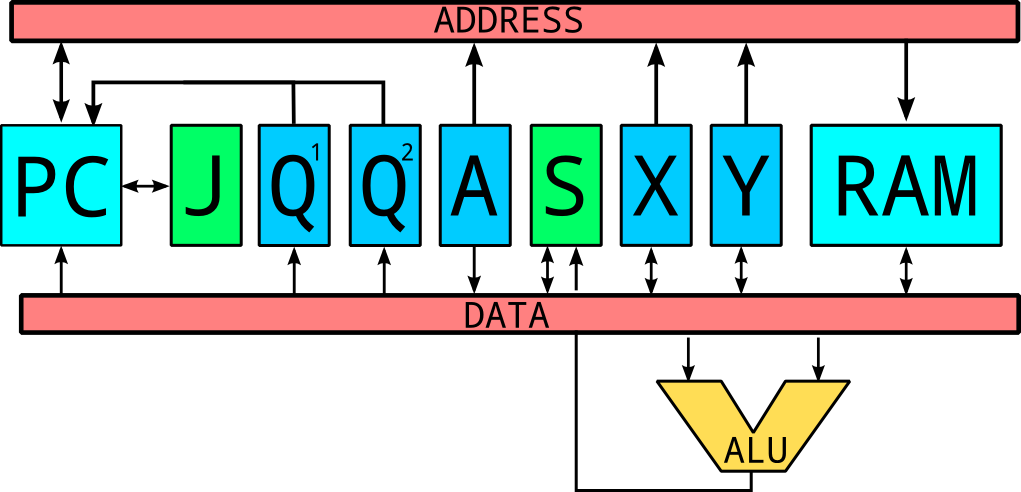
\includegraphics[width=\textwidth,height=\textheight,keepaspectratio]{Dataflow.png}
\caption{Dataflow diagram of the FML machine}
\end{figure}       

Now this image might be a little bit confusing. One should consider the two read
rectangles DATA and ADDRESS as ``viritual buses''\textsuperscript{\cite{bus}}.
One can interpret the picture as: X can both read and write from other components and be used for addressing.
Below will follow brief descriptions of the components. More indepth
descriptions are given in the appendix.

\begin{description}
  \item[X and Y] \hfill \\ 
  These are the two general purpose registers\textsuperscript{\cite{register}}
  which can be read, written to and used for addressing.
  \item[S] \hfill \\
  This is the general purpose stack. It can be both read and
  written to. Everytime some thing gets written to the stack it gets pushed onto the
  stack and everytime something is read from the stack the stack gets popped.
  The stack can not be used for addressing.
  \item[A] \hfill \\
  This is only a virtual register. It is read only and can be used for
  addressing. This is only used if an instructuion uses a non-register
  argument\footnote{A non-registry argument is a argument which is not any of
  the registers, the stack, or something from the memory. The value of A will
  (if used) be at the memory cell directly folowing the one at which the
  program counter is.}.
  \item[Q$^1$ and Q$^2$] \hfill \\
  These are the two interupt registers. These are very special and can only be
  written to. They will hold the addresses to which the machine should jump if an
  prepherial component makes a interupt request\textsuperscript{\cite{irq}}.
  
  \item[PC]\hfill \\
  This is the program counter. It keeps track on where in the memory the 
  instructions are being read from. It allso handles the both the subroutine
  jumps and the conditional breaking.
  \item[J]\hfill \\
  This is the jump stack. This stack is used to store the return addresses for
  subroutine jumps. This stack can only be manipulated by the program counter.
  \item[ALU]\hfill \\
  This is not really a ALU\textsuperscript{\cite{alu}}. The machine does not
  have a seppareta ALU component but this is just here to illustrate that the all of the components which can
  be read from can be used as arguments for arithmetic and logical operations.
  All of the results from the arithmetic and logical operations are always put
  on the stack.
  \item[RAM]\hfill \\
  This is the random access memory of the machine.
\end{description}

\subsubsection{Instruction Set Architecture}
The ISA\textsuperscript{\cite{ISA}} of the VM is built in a special but simple
fashion. Each instruction corresponds to a six digit integer 
where each digit corresponds to specific information regarding different types
of opcodes. The digits counting from right to left is: 

\begin{description}
  \item[First] Second argument
  \item[Second] First argument
  \item[Third] Arithmetic operations
  \item[Fourth] Logic operations
  \item[Fifth] Jump operations
  \item[Sixth] Special
\end{description}
This system of encoding information into each digit of the instruction makes the
implementation of the instruction decoder and the construction of the assembler
much easier.
It allows for all the operation types to be grouped into numerical ranges and it
gives  a lot of flexibility. Note that some of the instructions may be invalid
and some might be nonsensical but the instruction controler crashes if a invalid
instruction is encountered. The assembler is written in such a way that it can
only generate valid instructions\footnote{Allthough with the current
implementation of  the VM this is not necessairly true}.
So an example would be:
000401.
Where the 4 tells us that we should perform a modulo operation, 
the 0 says that the second argument is the \x register and the last 1 says 
that the first argument is the \y register. Notice that the order of
the last two digits is reversed in respect to the order of the arguments in
the operation.
This is due to a design choise made early in the design phase. It makes the
instructions code a bit more confusing to read but it makes the assembly code
become far more intuitive.\\
For a more detailed description of the ISA se the VM specifications in the
appendix.

\subsection{The components}
%Yo oskar det kan no g vara en bra ide att se över hela det här kalaset. Du
% kommer nog kunna fixa till det rätt bra imorgon när du e lite piggare.
We will now go through the general wokings of Components.sml, this file and
including functions are the structures of the Registers, Stack, Ram and Program
Counter, the functions are more specified in the appendix.

\subsubsection{Register}

Register is used in the implication for the VM as a 
register to save the values of x and y, to be able to 
handle all the different arithmetical operations. It can be increased or
decrease by one.

\subsubsection{Stack}
%Yo oskar!
%Det du har skrivit här om vad en stack är och hur den funkar är lite virrigt.
%skrev om det lite.
The stack handles the work progression with a LIFO\textsuperscript{\cite{lifo}}
structure this is a integral part of the VM implementation both to keep track of
return adresses and as a storage.

\subsubsection{Ram}
the ram memory works as a random access memory, it is set at a size 
at the start of the VM, and where we stores data in between operations.

\subsubsection{Program Counter}
The program counter handles the pointer to the memmory to see what is to be
done, as well handles the IRQ registers, the jumpstack as well as the
return jumps that redirects the pointer back to the original
address on the jump stack.
This is the main structure of the file all other structures are included in this
function

\section{Utillities}
For this program we have written some utillity files. The IO.sml and the
StringUtills.sml files just contains general helper funtions and thus play
little importance in the larger scheme of things. These two files will not be
described here.
\\
We will though give a shorter descrptions of the OpcodeResolve.sml file. This is
an important file since it works \footnote{It was supposed to work like this
but due to an implemtation fault in the VM it does not.} as a interface for both
the assembler and the VM. If both the assembler and the VM addheres to this
structure the assembler will not generate any instructions not accepted by the
VM. In general the \V+ResolveOpcode+ structure just contains a lot of ``lookup
tables'' in which one can find important information regarding the different
instructions and opcodes, such as which number corresponds to what type of operation, which 
arguments are allowed for each operations and so forth.
Since this structure was not propperly used in the VM implementation there are
still some things left to write for it, such as a series of reverse lookup
functions and checking for invalid instructions.

\section{Assembler}
\subsection{General}
The assembler which we have written for the FMl machine is a very basic yet
powerfull assembler. The assembler doesn't do much more than address
resolution, catching invalid opcodes and arguments. It allso enables the use of
both label pointers and value pointers. The main tasks of the assembler is the instruction code generation and
address resolution. The syntax of the assembler is inspired by the syntax for
the MOS 6510 assembly lanuage and primarily the syntax of the Turbo
Assembler\textsuperscript{\cite{tasm}} for the Commodore
64\textsuperscript{\cite{c64}}. The assembler is now fully functional and  we
dont see any need to augment it or redisgning any aspects of it. The assembler should only generate valid instructions but due to a major design error in the
implementation of the VM this is not neccesarily true any more. Below a short
example of a assembly program will follow:
\begin{verbatim}
% This a simple program which fills a part 
% of the memory with 100 consecutive integers
% trough rellative addressing.
#start
MOV 0 x
@start_address
MOV start_address y
#loop
MOV x $y
INC x
INC y
BLE x 100
JMP loop
HLT
\end{verbatim}
A line starting with a \V+#+ declares a label. The address of the label will
correspond to where in the code the the lebel gets declared.
A line starting with a \V+@+ declares a value. The address of the label will be
assigned independent of where in the code it apepars.
\\
\\
For a more indepth description of the assembly lanuage see the Assembler
part of the appendix.

\subsection{Implementation}
\subsubsection{General}
The assembler works in a fairly straight forward way. The first step in the
process of assembling is the lexical
analysis\textsuperscript{\cite{lexi}} in which the lines in the text file gets
tokenized. In this stage an ``intermediate structure'' \footnote{The use of the word structure here is a bit ambigous since it
actually is a structure in sml. But in this text it will reffere to an abstract
structure of data.} gets constructed.
This is an object which contains all of the labels, values and a list of the
tokenized lines. The list of the tokens contains tupels of
\verb+(label,offsett,token)+ wherer the lable is the last declared label and
the offset is how many addresses away from that line the current token is. All
of the labels and values will not be assigned an address in this phase. It is in
this phase where the opcodes and their arguments gets converted in to there
corresponding numerical instruction code. It is also during this phase in which
the syntax gets checked. If a syntax error is encountered the assembler will
stop emideatly. When the lexical analysis has been completed a check for
duplicate pointer declarations is performed.

The next phase in the assembly is the address resolution phase. This is done in
two phases, in the first one the labels gets resolved and in the second the
values gets  resolved. It begins by first resolving the labels.
This is done by first giving the assembler a \emph{base address} which is 
the address of the first label. As of now the first
non comment line in the input file has to be a label since every line has to
have a label assigned to it. Then the address resolving function continues
down the intermediate sturcture and remembers which line it is at and what it's
last read label was. When it runns into a new label-token it will set the new
label to it's current address and then continue on untill it has gone trough the entire
intermediate structure. After the labels have been resolved the assembler starts
to resolve the values. This is done in a very straightforward way. The assembler
just looks at the last address of the last entry in the output of the first
pass and looks at the last address, adds one to it and the just places all the
the values in after that address in the same order as they appeared in the file.
After all the addresses have been resolved the assembler runns trough the list
of tokens and replaces every pointer token with it's correct address.

After this is completed the assembler finalizes the code by converting
everything into a list of integers which then gets outputed to a file. And that
is how assembly code gets turned in to machine code.

The assembler runns in linear time with respect to the number of lines in the
code. This is under the assumption that the number of lines are far greater than
the number of values and labels in the code. This is a safe assumption for any
resonably written code. We se no need to try to optimize the performance of the
assembler.

\subsection{Intermediate Structure}
One of the most important parts of the assembler implementation is the
\V+Intermediate+ structure and especialy the \V+Inter+ datatype. There might
be some confusion regarding the \V+intermediate+ structure since it is a
sml structure which describes an abstract structure.It is in this datatype that
the tokenization of the code gets stored.
It composed of thre major components. The first is the \V+label_list+ in wich all of the label
declarations are stored. At first the address are set to \V+NONE+ this indicates
that their addresses have not yet been resolved. The \V+value_list+ works in the
same way as the \V+label_list+. Then we have the \V+token list+ wich is a list
of tupels of the form \V+(label_name, offsett, token)+. The \V+label_name+ is
the label wich is associated with the \V+token+. The assigned label will be the
last label declared before the \V+token+ is encountered. The \V+offsett+ is an
int corresponding to the distance from the assigned label that the token was
encountered. \V+offsett+ is vital in the address resolution of the tokens.


\subsubsection{Flow chart}
Below a flow chart will folow for how the assembler the assembles the
assembly code.
 
\begin{figure}[H]
\begin{centering}
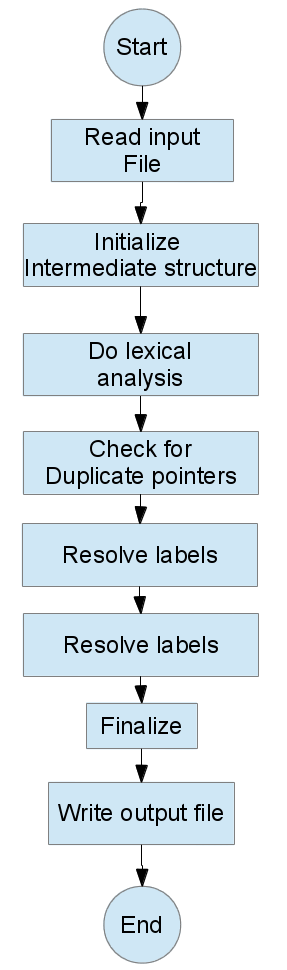
\includegraphics[width=\textwidth,height=\textheight,keepaspectratio]{assembler_flow.png}
\caption{Dataflow diagram of the assembler}
\end{centering}
\end{figure}

\newpage

\begin{figure}[H]
\begin{centering}
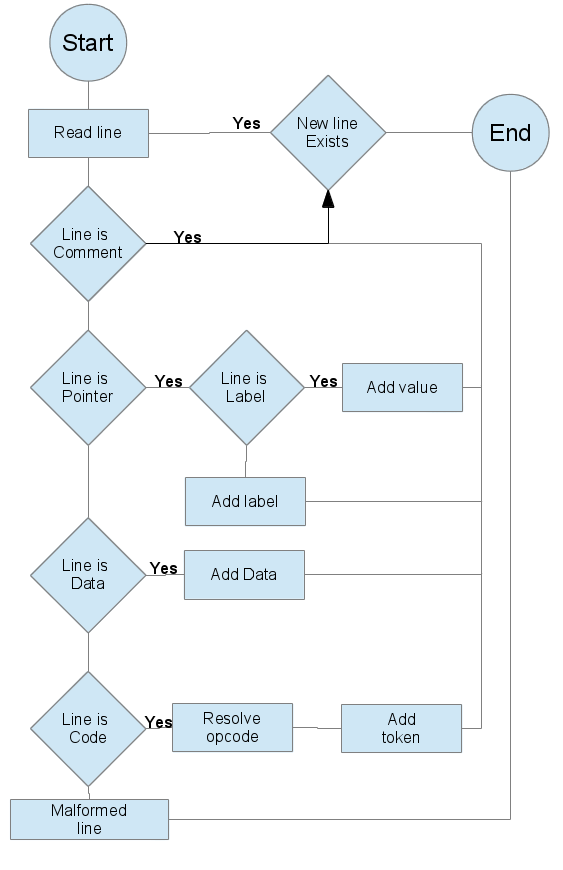
\includegraphics[width=\textwidth,height=\textheight,keepaspectratio]{lexicographical_flow.png}
\caption{Dataflow diagram of the tokenization phase}
\end{centering}
\end{figure}

\newpage

\begin{figure}[H]
\begin{centering}
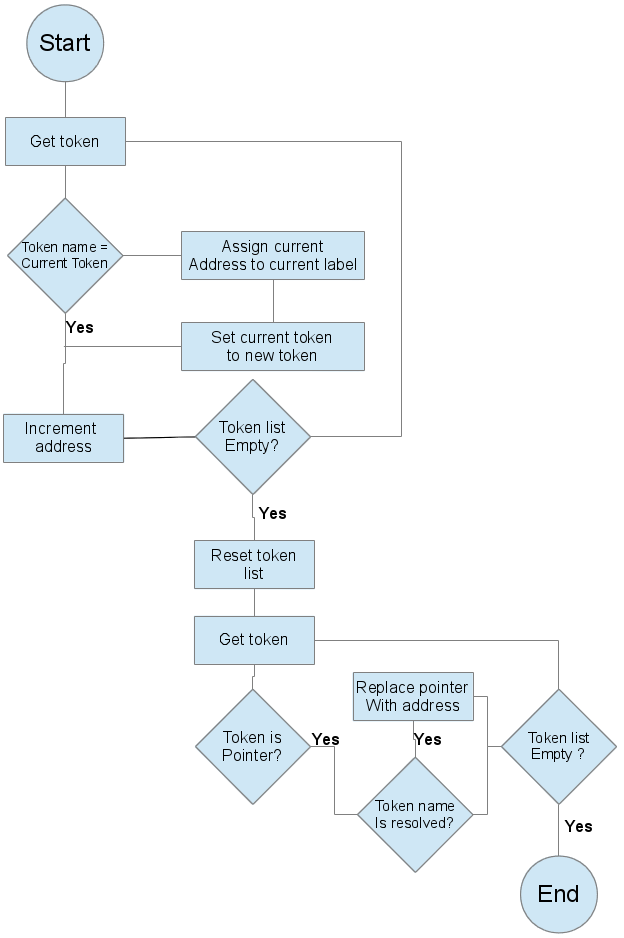
\includegraphics[width=\textwidth,height=\textheight,keepaspectratio]{address.png}
\caption{Dataflow diagram of the label address resolution}
\end{centering}
\end{figure}
\newpage
We have not included a flowchart for the address resolution of the values or
the finalization part since these are trivial.
\subsection{Usage}  
To use the assembler propperly one has to know how to write assembly code and
understand the detailed workings of the machine. We recomend studying both the
VM spcifications and the assembler documentation in the appendix before you
start to write programs for the machine.

The working of the assembler program is very straight forward. just write your
assembly code in a file called \V+in.asm+ and run the \V+Assembler.sml+ file in
the sml interperter of your choosing and if there are no errors encountered during
the assembling of the program the assembeled program will be outputed to a file
named \V+out.fml+.

\section{Summary}
In general this project has been a great sucssess considering the scale of the
project and the time constraints. We have designed a very sleak, efficient and
minimalistic VM. Even with it's minimal set of operations, programming for it is
much fun and quite straight forward compared to more complicated machine
lanuages. This is mainly due to the general purpose stack\footnote{Many of the
older 8-bit micro porcessors did not have a general purpose stack which made
programming for them somewhat cumbersome}.
We have managed to write a fully functional and fully featured assembler which
enables the writing of programs of unbounded complexity I.e there is no design
flaw in the assembler which would make it unpractical to write more elaborate
programs in it.
\subsection{Work to be done}
There are still a few untied strings to be tied up and folds to be flattened.
The VM implementation is as of now largley incomplete and only handles a small subset
of all the operations. It also needs to be rewritten in order to use the
\V+ResolveOpcode+ structure inorder to ensure compatibility with the assembler.

After the VM implementation is fully functional it would be nice to write some
prepherial components for handling output, input and timing.

And maybe one day we will write a high level lanuage for the machine.

After all of this is done and we have gotten permission from the lecturers the
entire project will be made avaliable as open source.
\subsection{Highlights}
What are we really proud of this project. First of all that we actually
did it\footnote{It contains roughly 1600 lines of code!}. Secondly the fact that
the VM is very minimalistic and yet powerful.
This is primarily due to the way the instruction are encoded into integers and
also trough the existence of the general purpose stack.

The assembler turned out much better than we had originaly imagined. And when
the \V+OpcodeResolve+ structure gets implemented propperly it will only generate
valid instructions.
\section{Appendix}
\subsection{VM specifications}
\subsubsection{Structure} 
The VM consists of 9 components. Two general purpouse registers(\x \ , \y ), one
general purpose stack (\s), One virtual read only register (\A), One jump stack
\J, Two IRQ address registers (\q \ , \qq), One ``ALU'', One program counter
(\pc) and of course a random acces memory.

\paragraph{The general purpose registers} \
\\
The two general purpose registers \x \ and \y \ are both capable of being used
for all arithmetic operations and their values can also be used as addresses.
These two registers can be incremented and decremented.

\paragraph{The stack} \
\\
The stack \s \ is a standard LIFO stack of unlimited size. The stack can not be
used for addressing. One can not read the top of the stack without popping it. If
one tries to get a value from an empty stack an exception will be raised and the
VM must halt.

\paragraph{The Argument Register} \
\\
Now this is just a virtual read only register. The argument \A \  is only
accesible if the instruction being executed takes a predefined argument. The
argument will be the value of the memory location after the location at which
the \pc \  is currently pointing. No well formed instruction should refere to
\A \ unless it is supposed to.

\paragraph{The Jump Stack} \
\\
The jump stack \J \ is not accesible by anything besides the \pc. The program
counter is of infinite size. The jump stack is responsible for keeping track
of the return address when a subroutine is performed. Every time someone
issues a subroutine jump the current address will be pushed onto the stack.
When a return jump is issued \J \ gets popped and it's value gets assigned to
the \pc. The top entry on the stack can not be accsessed without popping the
stack.
If someone tries to execute a return jump if the jump stack is empty a exception 
shall be raised and the VM must crash.

\paragraph{The IRQ registers} \
\\
The IRQ registers \q \ and \qq \ are two pointers to the memory. These are two
write only registers and can only be read by the \pc. The IRQ registers can be
assigned values like all the other registers.  If a interrupt is issued the \pc
\ will be assigned to the value of the corresponding IRQ register and the current
value of the \pc \ will be pushed onto \J.

\paragraph{RAM} \
\\
The RAM in this machine works pretty much like any other random access
memory. If any instruction tries to wrtie or read from addresses lying outisde
of the size of the ram the VM should crash.

\subsubsection{ISA}
Every opcode is represented by a integer where each digit provides
information about what the VM is to do in that step. The digits are from right
to left as follows.

\begin{description}
  \item[First] Read location
  \item[Second] Write location
  \item[Third] Arithmetic operations
  \item[Fourth] Logic operations
  \item[Fifth] Jump operations
  \item[Sixth] Special
\end{description}
Below is a table describing what each digit value corresponds to:
\begin{center}
\begin{tabular}{l || *{10}{c |}}
Value & 0 & 1 & 2 & 3 & 4 & 5 & 6 & 7 & 8 & 9 \\
\hline
Read & \x & \y & \s  &\mx & \my & \ma & \A & & & \\

Write & \x & \y & \s  &\mx & \my & \ma & \q& \qq & \A &\\

Arit &  & \V+INC+ & \V+DEC+ & \V+ADD+ & \V+SUB+ & \V+MUL+ & \V+DIV+ & \V+MOD+  & 
&
\\

Logic &  &  \V+EQL+ & \V+GRT+ & \V+LES+ & \V+BRL+ & \V+BRR+ & \V+AND+ & \V+ORR+
& \V+XOR+ & \V+NOT+\\

Jump & & \V+JMP+ & \V+BEQ+ & \V+BLE+ & \V+BGR+ & \V+JSR+ & \V+RET+ & & & \\

Special & & H & Se & \V+POP+ &  &  &  &  &  &  \\	
\end{tabular}
\end{center}
Here \mx , \my and \ma is to be read as address of \x , \y \ and \A.  All
arithmetic and logic operations operations writes their output to the stack.\\
Here some examples follows:\\
\verb+000042+ $\rightarrow$ Move value at \s \ to memory cell at the address
stored in \y. \\
\verb+000401+ $\rightarrow$ Get \x \ mod \y \ and write result to \s \\
\verb+020046+ $\rightarrow$ Skip next instruction if \my \ is equal to \A \\
\newpage

First I would like to  mention that
\verb+000000+ will be the \verb+NOP+ operation since it would translate to just
moving \x \ to \x \ . 
We can now group the instructions in to numerical ranges:

\begin{tabular}{l l}
  \V+000000+ & \V+NOP+ \\
  \hline
  \V+000001-000076+ & Move operations \\
  \hline
  \V+000100-000776+ & Arithmetic operations \\
  \hline
  \V+001000-009076+ & Logic operations \\
  \hline
  \V+010000-070000+ & Jump operations \\
  \hline
  \V+100000+ & Special \\
\end{tabular} \\
As is apparent from this list many values would yield invalid or
nonsense operations.
The instruction decoder must take this into consideration.

Below will follow specifications for all the instruction types.

\subsubsection{Instruction types}
Every instruction will take exactly one cycle. Almost every instruction needs
only one memory cell and should increment the \pc \  by one.
Any operation using  a argument I.e \A \ will occupy two memory cells and
increment the \pc \ by two.\\
Using jump operations may affect the \pc in other ways.
No operation except moves to the IRQ registers (\q \ and \qq ) are allowed.
If any other operation where to try to access the IRQ registers the opcode is
invalid and the VM should crash.

\paragraph{Move operations}\
\\
The only invalid move operations are those where the second digit is a 8 since
one can not write to \A.
Although some are nonsensical such as \V+000011+ since it would move \y \ to \y \ .

\paragraph{Arithmetic operations} \
\\
The increment($++$) and decrement($--$) operations only take one write argument
and the read argument should be ignored. Incrementing or decrementing a register
or memory cell updates the value stored in that registry directly and does not
affect any thing else.\\
The other arithmetic operations takes the write digit as the first argument to
the operation and the write operation will be the second argument.
The result of the operation is always stored on the stack.\\
If one tries division by zero a exception should be thrown and the VM shall
crash.

\paragraph{Logic operations} \
\\
The logic operations work in the same way as the arithmetic operations. The
comparison operations will return 0 if the result is false and 1 otherwise.
Any logic operation where the 3:d digit is non zero is an illegal instruction
and a exception should be thrown and the VM shall crash.

\paragraph{Jump operations} \
\\
The standard address jump (J) will jump the \pc \ to the address given by it's
read digit.\\
The conditional breaks takes the write digit as it's first argument and the read
digit as it's second argument. If the test fails the \pc \ will skipp the next
instruction. This will require som tricks to implement. The VM must , at
runtime, identify weather or not the following instruction takes up one or two
memory cells.\\

A \V+JSR+ (subroutine jump) will take a argument in \A \ and move the \pc \
there and it will also put it's current value on \J.\\
A return jump will jump to the address at the top of \J \ plus one or two
depending on weather a non register argument is used.
 \footnote{If the return jump where to return to the value at the top of the
 stack it where to return to the address where the subroutine jump is and thus 
 get stuck in a loop} and then pop the stack.If the jump where to be empty the 
 VM should crash and an exception should be raised.\\


\paragraph{Special}\
\\
The Halt operation which just stops the VM and
raises an exception.\\
And the \V+SEM+ or Stack empty operation which returns 1 if the stack is empty
and 0 else.
The \V+POP+ just pops the stack. I.e removing the top object.

\subsubsection{Opcodes}
Below a short summary of all the avliable opcodes will follow.\\
\begin{tabular}{l || c | *{7}{c|} | r}     
\textbf{Mnemonic} & \textbf{Description} & \x & \y& \s & \A &\ma & \mx & \my &
Args
\\
\hline
\V+NOP+ & No Operation & x & x & x & x & x & x & x & 0  \\ 
\hline
\V+MOV+ & Move operations & b & b & b & r & b & b & b & 1 \\
\hline
\V+INC+ & Increment& b & b & x & x & x & x & x & 1 \\
\V+DEC+ & Decrement	& b & b & x & x & x & x & x & 1 \\
\V+ADD+ & Add		& r & r & b & r & r & r & r & 2 \\
\V+SUB+ & Subtract	& r & r & b & r & r & r & r & 2 \\
\V+MUL+ & Multiply	& r & r & b & r & r & r & r & 2 \\
\V+DIV+ & Division	& r & r & b & r & r & r & r & 2 \\
\V+MOD+ & Modulus	& r & r & b & r & r & r & r & 2 \\
\hline
\V+EQL+ & Equal		& r & r & b & r & r & r & r & 2 \\
\V+LES+ & Less		& r & r & b & r & r & r & r & 2 \\
\V+GRT+ & Greater 	& r & r & b & r & r & r & r & 2 \\
\V+BRL+ & Rotate L	& r & r & b & r & r & r & r & 1 \\
\V+BRR+ & Rotate R	& r & r & b & r & r & r & r & 1 \\
\V+AND+ & And		& r & r & b & r & r & r & r & 2 \\
\V+ORR+ & Or 		& r & r & b & r & r & r & r & 2 \\
\V+XOR+ & Xor		& r & r & b & r & r & r & r & 2 \\
\V+NOT+ & Not		& r & r & b & r & r & r & r & 2 \\
\hline
\V+JMP+ & Jump		& r & r & x & r & r & r & r & 1 \\ 
\V+BEQ+ & Jump Equal& r & r & r & r & r & r & r & 2 \\
\V+BLE+ & Jump Less	& r & r & r & r & r & r & r & 2 \\
\V+BGR+ & Jump Greater& r & r & r & r & r & r & r & 2 \\
\V+JSR+ & Subroutine Jump& r & r & x & r & r & r & r & 1 \\
\V+RET+ & Return Jump& x & x & x & x & x & x & x & 0 \\
\hline
\V+HLT+ & HALT& x & x & x & x & x & x & x & 0 \\
\V+SEM+ & Stack Empty& x & x & w & x & x & x & x & 0 \\
\V+POP+ & Pop Stack& x & x & w & x & x & x & x & 0 \\
\end{tabular}






\subsection{Assembler usage guide}

In this part of the appendix a brief explanation of how the assembly lanuage
works is given here.
\subsubsection{Syntax}
The syntax for the assembly code is pretty straight forward. Each declaration is
written on a single line. There are a few reserved identifiers:

\begin{tabular}{|c | c| c |}
\hline
Indentifier & Name & Description\\
\hline
\V+%<text>+ & Comment  & Will be ignored by the assembler\\
\hline
\V+#<name>+ & Label & Declares a label called \V+<name>+ \\
\hline
\V+@<name>+ & Value & Declares a value called \V+<name>+\\
\hline
\V+:<data>+ & Raw input & Returns \V+<data>+ as is \\
\hline
\verb+$<a>+ & address & Derefferences \V+a+\\
\hline
\V+x+ & x & The \x \ register \\
\hline
\V+y+ & y & The \y \ register \\
\hline
\V+s+ & s & The stack \s \\
\hline
\V+q1+ & IRQ1 & The \q \ register\\
\hline
\V+q2+ & IRQ2 & The \qq \ register\\
\hline
\end{tabular}
\\
\\
The names given to \emph{label}s and \emph{value}s can contain any characters except for
whitespace ones.\\
Operations are declared in a straightforward approach as:\\
\V+<opcode> <arg1> <arg2>+ \\
which arguments are allowed are dependent upon the opcode.\\
Any non whitespace character can be used for names of labels and values.\\
Each file has to start with a label.

\subsubsection{Usage}
\paragraph{General} \ 
\\
One noteworthy thing to point out is the limitations on the arguments. Due to
limitations in the VM only one ``none registry'' argument can be used for any
operation. A ``non registry'' argument is one which is either a number or a
a pointer. Derefferencing a pointer is a registry operations so they are valid.
Below follows some examples:
\begin{verbatim}
#label
@value
MOV label value    This is not accepted
MOV $label $value  This is perfectly fine
MOV 10 value       This is invalid
MOV 10 $value      But this is
ADD 1 10           This is invalid
ADD $1 $10         This is valid
ADD 1 $1           So is this
\end{verbatim}

\paragraph{Registers} \ 
\\
The useage of the registers is pretty straight forward. One has to remeber that
\V+q1+ and \V+q2+ are write only registers and that \V+s+ cant be used for
addressing so \verb+$s+ is not allowed and will generate a \verb+syntax+ error.
It is also good to keep in mind that all operations reading from the stack will
consume what is on top of the stack.

\paragraph{Pointers} \
\\
Using pointers is fairly straight forward. Alltough one has to keep in mind how
the addresses are resolved. All pointers will be resolved after the
tokenazation fo the code. First the \emph{labels} will be resolved and then the
\emph{values}.
This means that the first \emph{value} will lie after the last line of code. Since the
address of a \emph{label} depends on where in the code their addresses are easy to
reason about. However for \emph{values} things are bit different. Since vlues
will be given addresses which are ``independent'' of where in the code they appear it is
hard to reason about the address of a \emph{value}. Although the \emph{value} pointers are
resolved in order the first \emph{value} declared whill lie intermediatley after the
last line of code and the last \emph{value} declared will lie ``at the end'' of the
memory used by the program. This can be exploited to use rellative addressing.
Allthoug great care has to be taken.

it's important to remember that all pointers are reffered to troughout the entire
program therefor it's not allowed to define two pointers with the same name. If
this where to be allowed it would generate unpredictable behaviour so instead
the assembler will return a \V+assembler+ error.

\emph{label}s and \emph{value}s are interchangable. Since opcodes takes pointers as arguments
and has no idea weather or not they are \emph{label}s or \emph{value}s. From this the need for
caution arises. Since one can use \emph{value} pointers as arguments to jump operation
like this:
\begin{verbatim}
@bad_idea
ADD x y
MOV s x
MUL x y
JMP bad_idea
\end{verbatim}
Since it is not known what where \V+bad_idea+ points jumping to it is suicidal.

Since pointers are just numbers under the hood one needs to take into account
weather or not one uses them for their address orr for their \emph{value}s. Here is some
examples
\begin{verbatim}
@pointer
% This stores x in pointer
MOV x value
% This stroes x in the address which is
% stored at pointer
MOV x $value
% This adds one to the value stored at 
% pointer
ADD $pointer 1
% This adds one to the address of pointer
ADD pointer 1
\end{verbatim}

Pointers are imutable and once they has been declared they can not be changed.
One has to do some tricking to achive relative addressing using \emph{labels} or
\emph{values}.


\paragraph{Labels} \
\\
\emph{Labels} are declared using the \V+#+ identifier.
\emph{Labels} are resolved first and their addresses
correspond to location in the code where they are written. For example:
\begin{verbatim}
MOV x y
#loop
INC x
MOV x s
JMP loop
\end{verbatim}
In this code \V+loop+ points to the address where \V+INC x+ is stored. In the
tokenization of the assembly code the lines where a pointer is defined will be
ignored and the address where the next instruction or raw entry occurs. This can
lead to that poorly written code becomes ambigous. For example:
\begin{verbatim}
MOV x y
#loop
#silly
INC y
\end{verbatim}
Here \V+loop+ and \V+silly+ will both point to the same address which is silly.

Because tokenaization of the code happens before the address resolving a \emph{label}
will be ``in scope'' troughout the enitre code. So this code is perfectly valid:

\begin{verbatim}
MOV x y
JMP ahead
INC x
ADD x y
#ahead
ADD s x
\end{verbatim}
The \V+JMP ahead+ will jump to \V+ADD s x+ even though the \V+ahead+ flag is
defined after the jump. This was not a concious design choise but it is actually
quite usefull since one can define subroutines anywhere in the code which can be
accesed form anywhere in the code.\\
One possible piffall arises due to the fact that the assembler does not know the
difference between a \emph{label} and a \emph{value} after their addresses has been resolved.
So this code is valid assembly code:
\begin{verbatim}
#loop
ADD s x
MOV s $loop
JMP loop
\end{verbatim}
Allthough what this will do is that it will change what is at the address of
\V+loop+. But there \V+ADD s x+ lies! This is what is known as self-modifiying
code and it's the spawn of satan and should be avoided like one avoids Miami
beach during spring break. Allthough in some cases the interchangability of
\emph{value} and \emph{label} can be verry usefull if one wants to have ``arrays'' in ones
code. This is easily achived like this:
\begin{verbatim}
#array
:0
:1
:2
:3
\end{verbatim}
Here \V+array+ can be used as a pointer to the array. One can then manipulate
the array trough using rellative arressing of \V+array+ like this:
\begin{verbatim}
ADD 2 array
MOV s y
MOV 5 $y
#array
:0
:1
:2
:3
\end{verbatim}
This code would change the 2 into a 5. But great care needs to be taken since
one could easily end up outside of the ``array'' and corrupt the program.

\paragraph{Values} \ 
\\
\emph{Value}s are far more straight forward than \emph{label}. One only has to
take into account that what address a \emph{value} is given is somewhat
independet of where in the code it gets defined.

\paragraph{Jumping} \
\\
Doing oridary jumps using the \V+JMP+ operation is very straight forward. The
machine will just jump to the address given to the \V+JMP+ operator.

But for conditional branching things become a little bit less obvious. If the
test given to a conditional test fails the machine will skip the next
instruction. Letts illustrate this with a few examples:
\begin{verbatim}
MOV 10 x
BLE x 2
JMP this_does_not_happen
BGR x 2
JMP this_happens
\end{verbatim}

Subroutine jumps work in a very straight forward fashion. You just make a
subroutine call using \V+JSR <address>+ and then you use the \V+RET+ operations
to return to the address imediatley after the one from which the jump was
issued. One has to be carefull not to execute a \V+RET+ jump unless one has
actually made a subroutine jump. The VM will crash if a return jump is issued
and the jump stack is empty.

\paragraph{Arithmetic and logic operations} \
\\
The arithmetic and logic operations are quite straight forward. The arguments
given to the operations appear as they would in the normal case. So \V+ADD x y+
is x+y and \V+MOD x y+ is x mod y. All of these operations (except for \V+INC+
and \V+DEC+) store their result on the stack.

\subsection{Componets.sml description}
Due to misscomunication a radicaly diffrent description of how the
Components.sml file works was written and have been included here as an
appendix.
\subsubsection{Introduction}

The following structures and signatures are present in Components.sml are the
Ram, Stack, Register and ProgramCounter.

\subsubsection{The Ram structure}
\paragraph{Synopsis} \ 
\\
signature RAM\\
structure Ram :\textgreater RAM\\

The Ram structure provides a base of the functions of a ram memory. This
structure acts as something akin to a ``monad''. It hides all of the sidefects
sued for the array handling.

\paragraph{INTERFACE} \ 
\\
    type memory = int array
	\\val initialize : int $\rightarrow$ memory 							
 	\\val getSize : (memory) $\rightarrow$ int 
    \\val write :(memory * int * int ) $\rightarrow$ memory	  				
	\\val read : (memory * int) $\rightarrow$ int							
	\\val load : (memory* int list) $\rightarrow$ memory					
	\\val writeChunk : (memory * int * (int array)) $\rightarrow$ memory
	\\val readChunk : (memory * int * int) $\rightarrow$ int array			
	\\val dump : memory $\rightarrow$ string
\paragraph{Description} \
\\
val initialize : int $\rightarrow$ memory \\	
	Initialize the ram to a memory with the size of int, when int > 0
\\
val getSize : (memory) $\rightarrow$ int\\
		Gets the size of the memory
\\
val write :(memory * int * int ) $\rightarrow$ memory\\
		write takes a memory and writes a new value of int at the pointer of the first
		int and returns the memory
\\
val read: (memory * int) $\rightarrow$ memory\\
		read takes a memory and reads the value of the place of int
\\
val load: (memory * int list) $\rightarrow$ memory\\
		load takes a list of values and loads them to the memory
\\
val writeChunk: (memory* int *( int array)) $\rightarrow$ memory \\
		writeChuck takes a memory and a start pointer and adds a chunk to the memory
\\
val readChunk: (memory * int *int) $\rightarrow$ int array \\
		readChumk takes a memory and reads a chunk form first int to the last int and gives the values as an int array
\\
val dump: memory $\rightarrow$ string\\
		dump takes a memory and returns the value as strings

\subsubsection{The Stack structure}
\paragraph{Synopsis}\
\\
signature STACK \\
structure Stack :\textgreater STACK
\\
The Stack structure provides a base for the stack part of the Pc structure.

\paragraph{INTERFACE}\
\\
	datatype stack = Stack of (int list)\\	
	val empty : stack \\
	val push : stack * int $\rightarrow$ stack\\					
	val pop : stack $\rightarrow$ stack\\						
	val top : stack $\rightarrow$ int\\						
	val isEmpty : stack $\rightarrow$ bool \\						
	val dumpStack : stack $\rightarrow$ string\\					 
	
\paragraph{Description}\
\\
	val empty : stack\\
		is a definition of a empty Stack
\\
	val push : stack * int $\rightarrow$ stack\\					
		takes a stack and adds the value of int to the stack.
\\
	val pop : stack $\rightarrow$ stack	\\					
		takes a Stack and pops the first element of the stack.
\\
	val top : stack $\rightarrow$ int\\							
		takes the stack and returns the first element of the stack
\\
	val isEmpty : stack $\rightarrow$ bool\\						
		takes a stack and checks if it is empty if it is then true else false.
\\
	val dumpStack : stack $\rightarrow$ string\\
		takes a stack, then pops the stack until it's empty and returns all values as string

\subsubsection{The Register structure}
\paragraph{Synopsis} \
\\
signature REGISTER\\
structure Register :> REGISTER\\
\\
The Register structure provides a base structure of the different register that
is contained in the Pc as well the Virtual machine. The vm has two different registers.\\
\paragraph{INTERFACE} \
\\
	datatype reg = Reg of int 
\\	
	val setData : (reg * int) $\rightarrow$ reg 				
\\	val getData : reg $\rightarrow$ int						
\\	val increment : reg $\rightarrow$ reg						
\\	val decrement : reg $\rightarrow$ reg						
\\	val dumpRegister : reg $\rightarrow$ string
\paragraph{Description} \ 
\\

	val setData : (reg * int) $\rightarrow$ reg\\
		Setups a new Register \\
	val getData : reg $\rightarrow$ int	\\
		Gets the value of the reg as an int\\					
	val increment : reg $\rightarrow$ reg\\		
		Takes a reg and increment it with one.\\	
	val decrement : reg $\rightarrow$ reg\\					
		Takes a reg and decrements it with one.\\
	val dumpRegister : reg $\rightarrow$ string\\
		Takes the register and adds all elements to a string.\\

\subsubsection{The Program Counter structure}
\paragraph{Synopsis} \ 
\\
signature PROGRAM_COUNTER\\
structure ProgramCounter :> PROGRAM_COUNTER\\
\\
The ProgramCounter structure controls the execution flow of the VM
\\
\paragraph{INTERFACE} \ 
\\
	datatype pc = Pc of (int * Stack.stack * Register.reg * Register.reg)
\\
	val incrementPointer : (pc * int) $\rightarrow$ pc\\
	val jump : (pc * int) $\rightarrow$ pc\\
	val subroutineJump : (pc * int) $\rightarrow$ pc\\ 						
	val return : pc $\rightarrow$ pc\\	
    val interrupt : (pc * int) $\rightarrow$ pc\\
    val dumpPc : pc $\rightarrow$ string\\
\\
\paragraph{Description} \ 
\\
	val incrementPointer : (pc * int) $\rightarrow$ pc\\
		Takes a Pc and adds a int > 0\\							
	val jump : (pc * int) $\rightarrow$ pc\\
		Takes a Pc and jumps the pc counter to the value of int > 0\\
	val subroutineJump : (pc * int) $\rightarrow$ pc\\
		Takes a Pc and preforms SubrutineJump with the value of  int > 0 and adds the  value of the pointer + 1 to the stack\\						
	val return : pc $\rightarrow$ pc\\
    	Takes a pc and gets the value from the pointer and pops the stack with the value\\
	val interrupt : (pc * int) $\rightarrow$ pc\\							
		if the value of a is 1 or 2, then the value of i is added to s\\
	val dumpPc : pc $\rightarrow$ string\\
		Takes a pc and dumps the content of the pc as a string (the Pc contained a pointer, Stack, and tow registers)\\




\newpage
\begin{thebibliography}{}

\bibitem{Virtual}
{\url{http://en.wikipedia.org/wiki/Virtual_machine}\\
Retrieved: \today}

\bibitem{risc}
{\url{http://en.wikipedia.org/wiki/RISC}\\
Retrieved: \today}

\bibitem{6510}
{\url{http://en.wikipedia.org/wiki/6510}\\
Retrieved: \today}

\bibitem{z80}
{\url{http://en.wikipedia.org/wiki/Z80}\\
Retrieved: \today}

\bibitem{ISA}
{\url{http://en.wikipedia.org/wiki/Instruction_set_architecture}\\
Retrieved: \today}

\bibitem{Async}
{\url{http://en.wikipedia.org/wiki/Asynchronous_Processor#Asynchronous_CPU}\\
Retrieved: \today}

\bibitem{git}
{\url{http://en.wikipedia.org/wiki/Git_(software)}\\
Retrieved: \today}

\bibitem{bitbucket}
{\url{http://bitbucket.org}\\
Retrieved: \today}

\bibitem{pure}
{\url{http://en.wikipedia.org/wiki/Functional_purity}\\
Retrieved: \today}

\bibitem{7400}
{\url{http://en.wikipedia.org/wiki/7400}\\
Retrieved: \today}

\bibitem{opcode}
{\url{http://en.wikipedia.org/wiki/Opcode}\\
Retrieved: \today}

\bibitem{neuman}
{\url{http://en.wikipedia.org/wiki/Von_Neumann_architecture}\\
Retrieved: \today}

\bibitem{bus}
{\url{http://en.wikipedia.org/wiki/Data_bus}\\
Retrieved: \today}

\bibitem{register}
{\url{http://en.wikipedia.org/wiki/Register_(computing)}\\
Retrieved: \today}

\bibitem{irq}
{\url{http://en.wikipedia.org/wiki/Interrupt_request}\\
Retrieved: \today}

\bibitem{alu}
{\url{http://en.wikipedia.org/wiki/Arithmetic_logic_unit}\\
Retrieved: \today}

\bibitem{assembler}
{\url{http://en.wikipedia.org/wiki/Assembler_(computing)#Assembler}\\
Retrieved: \today}

\bibitem{c64}
{\url{http://en.wikipedia.org/wiki/Commodore_64}\\
Retrieved: \today}

\bibitem{tasm}
{\url{http://turbo.style64.org/}\\
Retrieved: \today}

\bibitem{lexi}
{\url{http://en.wikipedia.org/wiki/Lexical_analysis}\\
Retrieved: \today}

\bibitem{lifo}
{\url{http://en.wikipedia.org/wiki/LIFO_(computing)}\\
Retrieved: \today}
\end{thebibliography}

\end{document}
